\documentclass[11pt]{article}
\usepackage{geometry}
\geometry{letterpaper, margin=1in}
\usepackage[utf8]{inputenc}
\usepackage{graphicx}
\usepackage{upgreek}
\usepackage{url}
\usepackage[T1]{fontenc}
\usepackage{amsmath}
\usepackage{minted}
\usepackage{scalerel}
\usepackage[colorinlistoftodos]{todonotes}
\usepackage[
backend=biber,
style=ieee,
sorting=none 
]{biblatex}
 
\addbibresource{refs.bib}

\title{ECE532S Digital Systems Design \\ \vspace{0.4cm}
       \Large Tutorial 4 - Debugging on Board Using the ILA \\ \vspace{0.4cm}
       \small Last Updated: Jan, 2021}
\author{ }
\date{ }


\begin{document}
\maketitle
\vspace{-1cm}

When designing hardware systems on FPGAs, it is not always possible to debug all issues using simulation. Sometimes we encounter issues that only present themselves once the bitstream is downloaded onto the FPGA, and sometimes we need to test things at a scale that would be intractably long to simulate. In these cases, we turn to using debug hardware cores that allow us to capture information about the actual hardware as it runs on the FPGA. In this tutorial, we'll be introducing one such core and applying it to some hardware design to see how it could be used to assist in debugging.

The \textit{Integrated Logic Analyzer}, or \textit{ILA} for short, is a Xilinx debug core that can capture the values of probed signals and then display those values on a waveform viewer within the Vivado environment. A "probed" signal is a wire that is connected to the ILA, without disturbing the existing connections to that signal; i.e. the ILA simply watches the values of that signal. Figure~\ref{fig:ila} shows the block diagram for the ILA, taken from the ILA product guide~\cite{xilinx_ila}. The core contains a number of probes, a clock signal at whose edges the data is captured, and some trigger signals. The probes are the signals to be captured, and the trigger signals determine when we start capturing a new set of data. Note, the probe signals themselves can be used to trigger the ILA, so we usually don't include the trigger signals in our instantiations of the ILA. More details will be covered later in the tutorial.


\begin{figure}[!h]
    \centering
    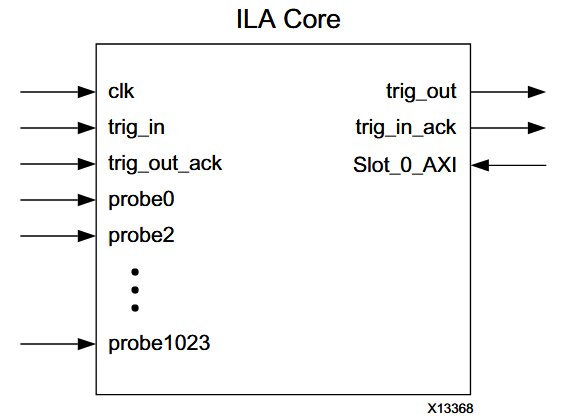
\includegraphics[width=0.4\textwidth]{images/ila.png}
    \caption{ILA block diagram}
    \label{fig:ila}
\end{figure}




\section{Marking Nets as Debug}
\label{sec:mark_as_debug}
There are two ways in which we can insert an ILA into a project. The first method is an automated insertion methodology used through the annotation of HDL source files, and the second is the actual instantiation of an ILA in IP Integrator view. The ILA Core instantiation will be covered in Section~\ref{sec:ila_core}, and here we will discuss the debug flow available in Vivado for HDL source files.

\textbf{Create} a new Vivado project according to the steps in previous tutorials, making sure to add the \textit{tutorial.v} and \textit{tutorial.xdc} files as a source and constraint file respectively. 
%Feel free to select the device by part number or by selecting the board file installed in tutorial~3. In any case, we still need to add the constraint file since the board file cannot be used to specify constraints outside of the IP Integrator view. 
The contents of \textit{tutorial.v} are shown in Figure~\ref{fig:led_shift_app}.

\begin{figure}[!h]
\centering
\begin{minted}
[
frame=lines,
framesep=2mm,
baselinestretch=1.2,
bgcolor=white,
fontsize=\footnotesize,
linenos,
breaklines,
]
{verilog}
module tutorial (
    input clk,
    input reset,
    input [7:0] swt,
    output [7:0] led
    );

	wire direct_connect = swt[7];
	wire [7:0] out_value;

	//Counter
	wire[26:0] count_limit = {swt[6:0],20'd0};
	reg [26:0] counter;

	always @(posedge clk) begin
		if(reset) begin
			counter <= 27'd0;
		end else if(counter == count_limit) begin
			counter <= 27'd0;
		end else begin
			counter <= counter + 1;
		end
	end

	//Shift LED values
	reg [6:0] led_shift;

	always @(posedge clk) begin
		if(reset) begin
			led_shift <= 7'b0000001;
		end else if(counter == count_limit) begin
			led_shift <= {led_shift[5:0],led_shift[6]};
		end
	end

	//Output
	assign out_value = {direct_connect,led_shift};
	assign led = out_value;

endmodule
\end{minted}
\vspace{-0.7cm}
\caption{Simple verilog module to shift output of LEDs with a counter}
\label{fig:led_shift_app}
\end{figure}


\noindent
The \textit{tutorial} module is the top level module of the project, and it's input and output signal names should match those of the added constraints file. The module takes the switch values as input, and output some value to the LEDs. The most significant switch value is connected directly to the most significant LED, while the other switches are used to determine at which value some counter is to reset. Specifically, the lower 7 bits of the switches determine the number of $2^{20}$ cycles some counter should count to before resetting. Recall that our clock frequency is 100MHz, so a value of 100 on the switches should be approximately one second. Each time the counter resets, the values output to the lower LEDs is rotated to the left by one. In effect, the switches determine the rate at which some pattern sifts through the LEDs. The pattern is fixed at 0000001 in binary. Note, the reset signal is active low.

To monitor some of these signals after we download the system onto the FPGA, we need to mark the signals in question \textit{as debug}. There are a number of ways to mark a signal as debug, and we'll cover a few of them. First, we can annotate the HDL itself to mark a wire or register output as debug. For verilog, the notation to mark the signal \textit{direct\_connect} as debug for example is the following:

\begin{minted}
[
framesep=2mm,
baselinestretch=1.2,
bgcolor=white,
breaklines,
]
{verilog}
    (* mark_debug = "true" *) wire direct_connect = swt[7];
\end{minted}

\noindent
Use this methodology and \textbf{mark} both the signal \textit{direct\_connect} and \textit{out\_value} as debug. Note, marking a signal as debug also prevents Vivado from optimizing a signal away, which can often happen in some of the optimization stages of Synthesis. Now run \textbf{Synthesis} for the project but do not proceed to \textit{Implementation} when \textit{Synthesis} completes. Instead, select \textbf{Synthesis $\rightarrow$ Open Synthesized Design} from the \textit{Flow Navigator} pane on the left side of the Vivado interface. From the drop down menu in the top right of the Vivado interface, select \textbf{Debug} to switch to the debug view (see Figure~\ref{fig:debug_view} for reference).

\begin{figure}[!h]
    \centering
    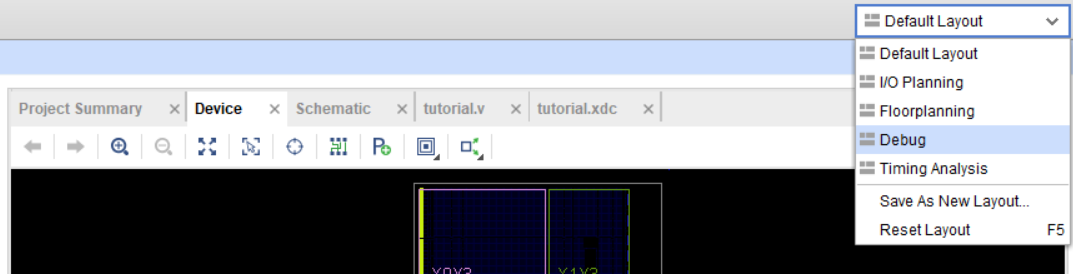
\includegraphics[width=0.9\textwidth]{images/debug_view.png}
    \caption{Selecting the Debug view from the open Synthesized Deign}
    \label{fig:debug_view}
\end{figure}

You should see the \textit{Debug} tab in the bottom window. Here are listed all nets that have been marked as debug in your design; check to make sure both of the signals we've marked for debug are listed here. See Figure~\ref{fig:debug_list} for reference. Note, the nets are listed under the \textit{Unassigned Debug Nets} heading, since these debug nets have not yet been connected to an \textit{ILA}.

\begin{figure}[!h]
    \centering
    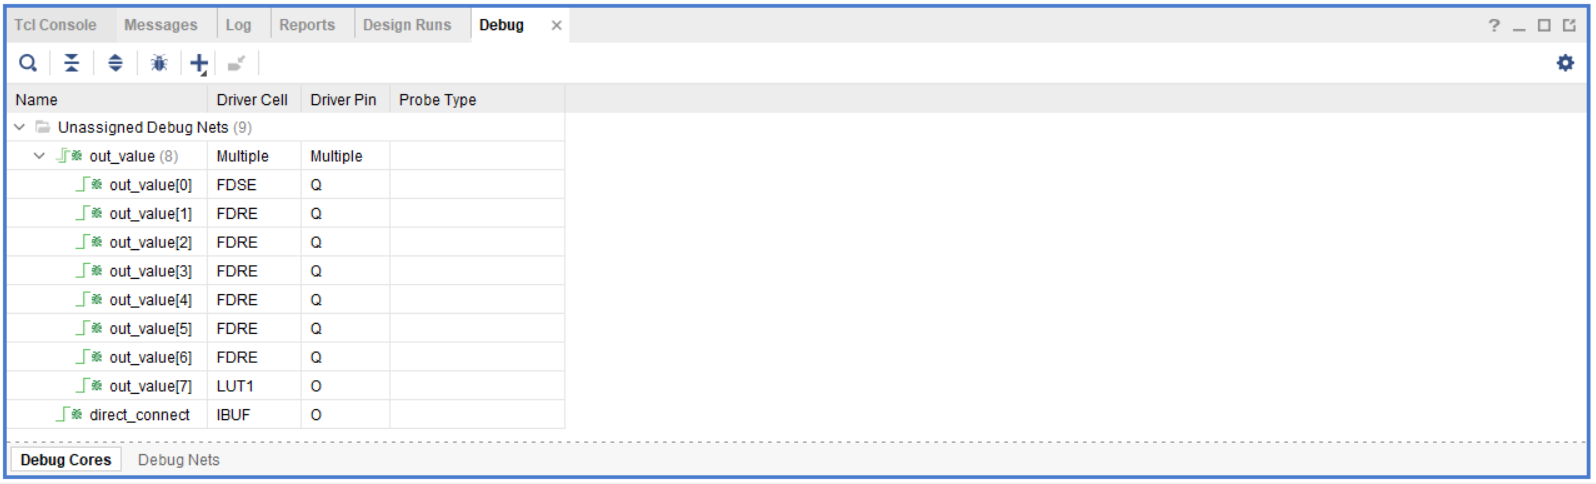
\includegraphics[width=0.9\textwidth]{images/debug_list.png}
    \caption{List of nets marked for debug}
    \label{fig:debug_list}
\end{figure}

We can also add more nets to the debug list from the \textit{Open Synthesized Design} view. In the \textbf{Netlist} window on the left, select the \textbf{Netlist} tab to see a list of all of the nets in your design. Note, this will not include any nets that have been optimized away during the recently executed \textit{Synthesis}. You can \textbf{right click} any of the nets listed here and select \textbf{Make Debug} to add the net to the list of debug nets. Find the net corresponding to the \textit{counter} signal and mark it as debug (see Figure~\ref{fig:counter_as_debug}). We should now have a total of three nets listed under the \textit{Unassigned Debug Nets} header in the \textit{Debug} tab. You can also mark a net \textit{as debug} using the TCL Console, though we won't be demonstrating that in this tutorial

\begin{figure}[!h]
    \centering
    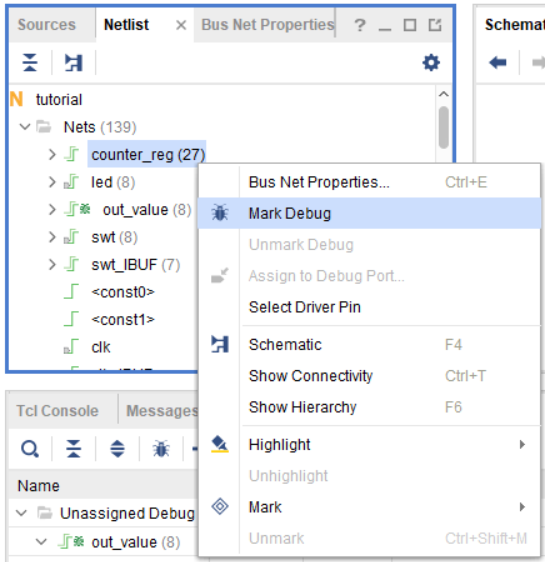
\includegraphics[width=0.6\textwidth]{images/counter_as_debug.png}
    \caption{Marking the counter register as debug}
    \label{fig:counter_as_debug}
\end{figure}




\section{Running the Debug Wizard}
\label{sec:debug_wiz}
In order to connect the nets we've marked as debug, we need to run the \textit{Debug Wizard}. To open the \textit{Debug Wizard}, select \textbf{Tools $\rightarrow$ Set Up Debug} from the Vivado window tool bar. Click \textbf{Next} on the first window to bring up the list of nets we've marked as debug (see Figure~\ref{fig:debug_wizard}). Each net is also listed with the associated clock, which is the clock used to sample the net. Some of the signals we've marked as debug are not synchronous signals, since they are combinational in nature, and as such have no clock selected by default. Our design has only one clock, so it should be used for all signals. \textbf{Right click} each signal without an associated clock, choose \textbf{Select Clock Domain...}, and select the only clock listed.

\begin{figure}[!h]
    \centering
    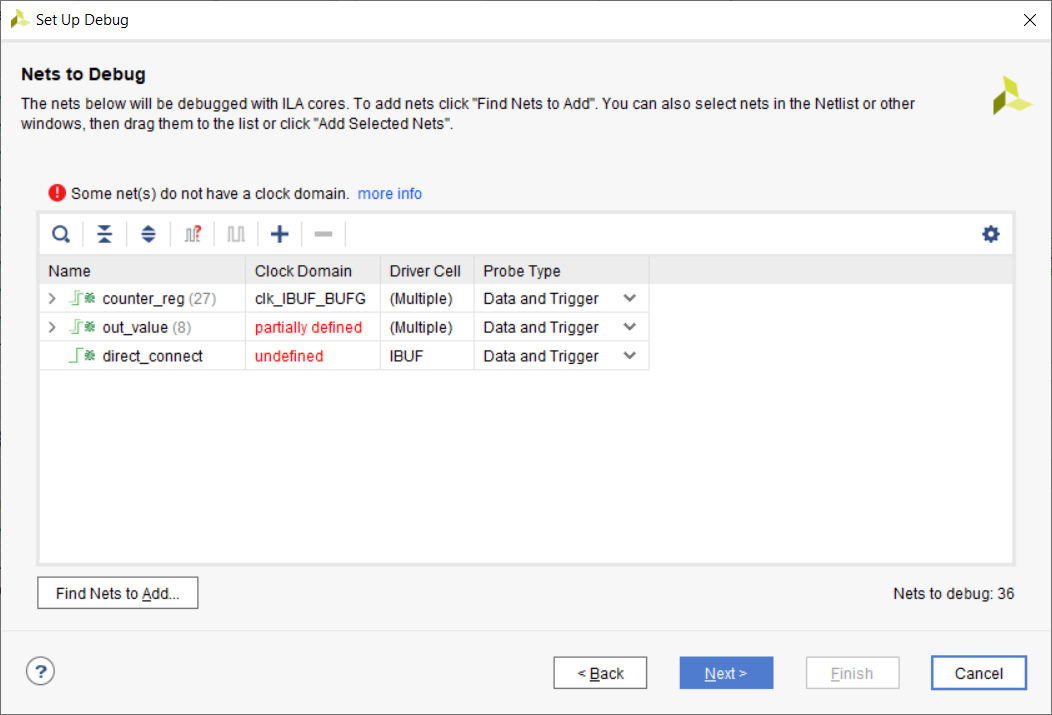
\includegraphics[width=0.9\textwidth]{images/debug_wizard.png}
    \caption{List of nets in the Debug Wizard}
    \label{fig:debug_wizard}
\end{figure}

\newpage
Click \textbf{Next} to advance to the \textit{ILA Core Options} menu. In this window, we can select the depth of our \textit{ILA} core, i.e. the number of samples of the probe signals that the ILA can store at a time. Also, the \textit{Input pipe stages} setting is important if the ILA is causing timing failures, as increasing pipeline registers can ease timing closure for the probed signals. Leave the \textit{Sample of data depth} at \textbf{1024} and click \textbf{Next} and then \textbf{Finish} to complete the \textit{Debug Wizard}. Check the \textit{Debug} tab again to see that an \textit{ILA} core has been added (named \textit{u\_ila\_0}, or something along those lines) that contains all of our debug nets. The \textit{Unassigned Debug Nets} listing should contain no nets at this time. See Figure~\ref{fig:debug_list2} for reference.

\begin{figure}[!h]
    \centering
    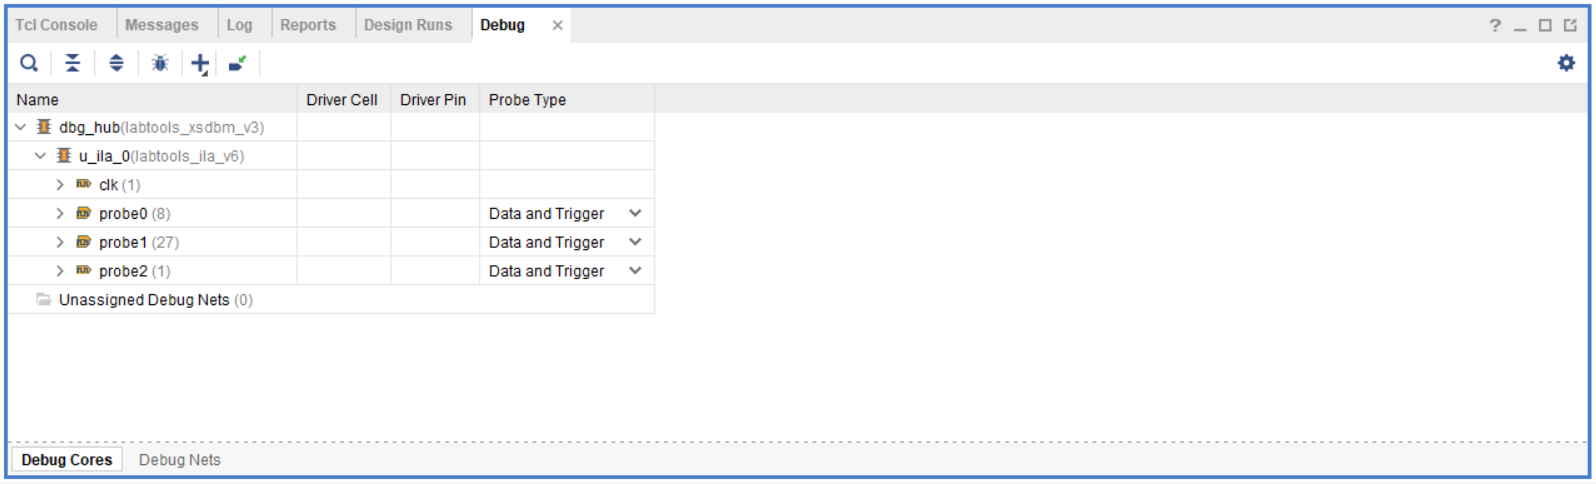
\includegraphics[width=0.9\textwidth]{images/debug_list2.png}
    \caption{List of nets marked for debug, after assignment to ILA cores}
    \label{fig:debug_list2}
\end{figure}




\section{Using the ILA in Hardware Manager}
\label{sec:hw_man}
Now that we've added the \textit{ILAs}, we can save the project (if asked, save additions to the constraints to the constraints file \textit{tutorial.xdc}), close the \textit{Synthesized Design}, and rerun \textbf{Synthesis}, \textbf{Implementation}, and \textbf{Generate Bitstream} to generate the final bitstream that includes the \textit{ILA}s. Open \textbf{Hardware Manager} and download the bitstream to the FPGA. Note, when selecting a bitstream to program the FPGA, you are also prompted to select a \textit{Debug probes file}. This file contains information about all of the debug cores in the design. This field should be populated automatically to the \textit{probes file} created when you generated the bitstream. See Figure~\ref{fig:select_bit} for reference.

\begin{figure}[!h]
    \centering
    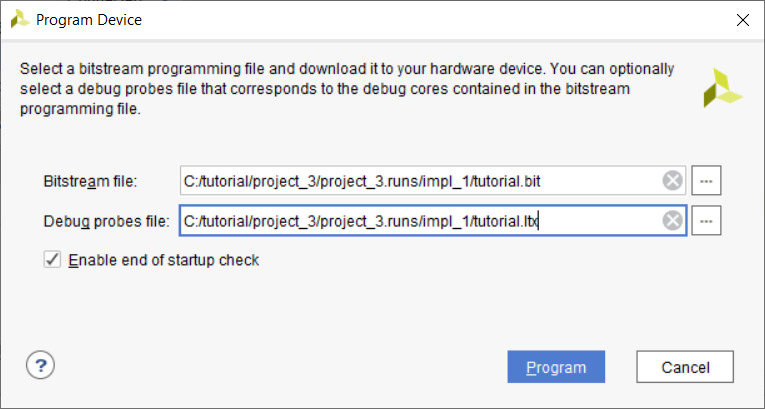
\includegraphics[width=0.8\textwidth]{images/select_bit.png}
    \caption{Selecting a bitstream and a probes file when programming the FPGA}
    \label{fig:select_bit}
\end{figure}

Once the FPGA has been programmed, all debug cores should be listed under the FPGA in the \textit{Hardware} window (see Figure~\ref{fig:hw_ila}). To open the ILA window, \textbf{double click} on the listed ILA, \textit{hw\_ila\_1} in our case. This should open the ILA interface in a new tab of the editor pane (though it may have been open already by default). The ILA interface is how we control the ILA and view the probed results. It is made up of three panes, depicted in Figure~\ref{fig:ila_interface}. The top window contains the waveform viewer, where the values of our probed signals are displayed. The bottom left window contains two tabs, with the ILA \textit{settings} and the ILA \textit{status}. And the bottom right window contains two tabs, for modifying the \textit{trigger} and \textit{capture} settings. The ILA we've implemented doesn't support capture settings, so only the trigger settings are of note for us.

\begin{figure}[!h]
    \centering
    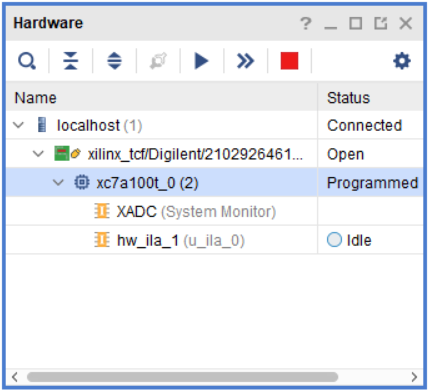
\includegraphics[width=0.45\textwidth]{images/hw_ila.png}
    \caption{The FPGA device with a single ILA core listed}
    \label{fig:hw_ila}
\end{figure}

\begin{figure}[!h]
    \centering
    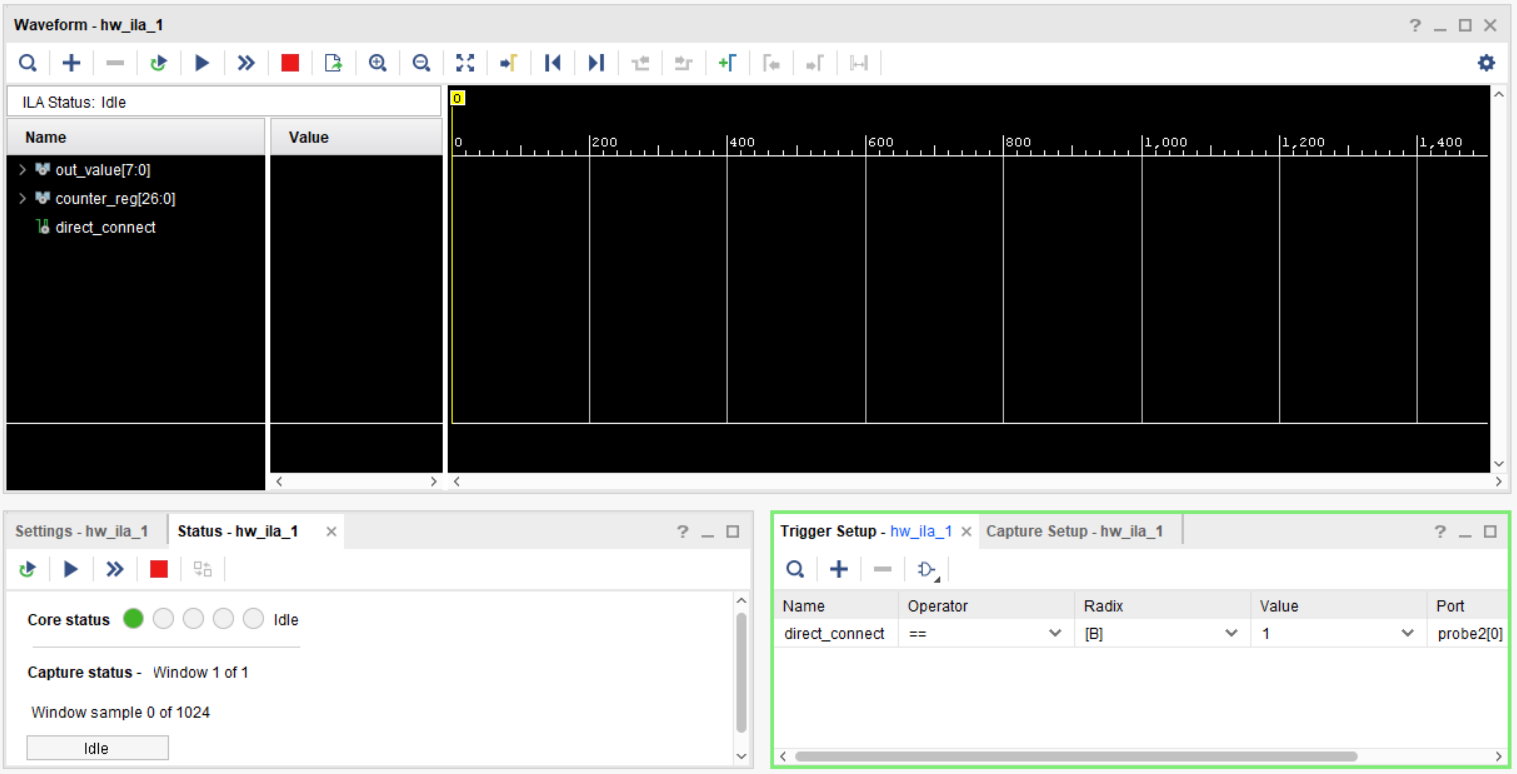
\includegraphics[width=0.9\textwidth]{images/ila_interface.png}
    \caption{The ILA interface within Hardware Manager}
    \label{fig:ila_interface}
\end{figure}

To setup the \textit{ILA}, first we'll modify the settings, \textbf{open} the settings tab. The main setting of note for our purposes is the \textit{Trigger position in window}. This setting determines at which position within the captured data the trigger event occurs. Earlier in the tutorial we mentioned that the \textit{ILA} starts capturing data when the trigger is encountered. In reality, the \textit{ILA} continuously saves the probed data in a circular buffer buffer fashion, i.e. the newest probed data saves over the oldest data already stored. When a trigger is encountered, the \textit{ILA} stops saving probed data once enough data has been stored such that the trigger event appears in the position indicated by the \textit{Trigger position in window} setting. Leave this value at the default setting of \textbf{512}.

Next, we focus on the \textit{Trigger} settings. Here, we setup what condition triggers a capture event. Press the 
~\scalerel*{
\includegraphics{images/add_probe.png}}{(}~
button to add a new probe to our triggers, and select \textit{direct\_connect} from the list. Next, we decide what specific condition on our trigger signal indicates a trigger event. We set the \textit{Operator} field to \textbf{==} and set the \textit{Value} field to \textbf{1 (logical one)}, which will setup a trigger event when \textit{direct\_connect}, a.k.a. swt[7], equals logical one. Note, we could also set the \textit{Value} to \textit{R} if you want a rising edge to trigger an event. If we have multiple trigger signals, the
~\scalerel*{
\includegraphics{images/global_trigger.png}}{(}~
button determines how to combine the different trigger event values; select the \textbf{global AND} option, which will trigger when all of the conditions are met (whereas the \textit{global OR} will trigger when any of the conditions are met). For our single trigger condition, either option will work equally well.

Now that we've set our trigger, we need to run the \textit{ILA}. Open the \textit{status} tab to observe that the current status is \textit{Idle}. \textbf{Push} all the switches on your board to the zero position, and then press the
~\scalerel*{
\includegraphics{images/run_ila.png}}{(}~
button to \textit{Run} the \textit{ILA}, where it waits for the trigger event.
The status bar in the lower part of the \textit{status} tab should show that the \textit{ILA} is 49\% full, since we set our trigger position in the middle of our window. \textbf{Push swt[7]} up to trigger the event. The status should change quickly to \textit{Full} and then \textit{Idle} again. The waveform view should show the captured values now, as shown in Figure~\ref{fig:ila_waveform}. The marker labelled with a \textit{T} shows where the trigger event occurred. If you zoom into the waveform, you should notice that the output values change every cycle, since we set the switches to zero. So even though we can't see the LEDs changing, they are in fact changing values. Try different values of the switches and re-Run the \textit{ILA} to verify that the counter works as expected.

\begin{figure}[!h]
    \centering
    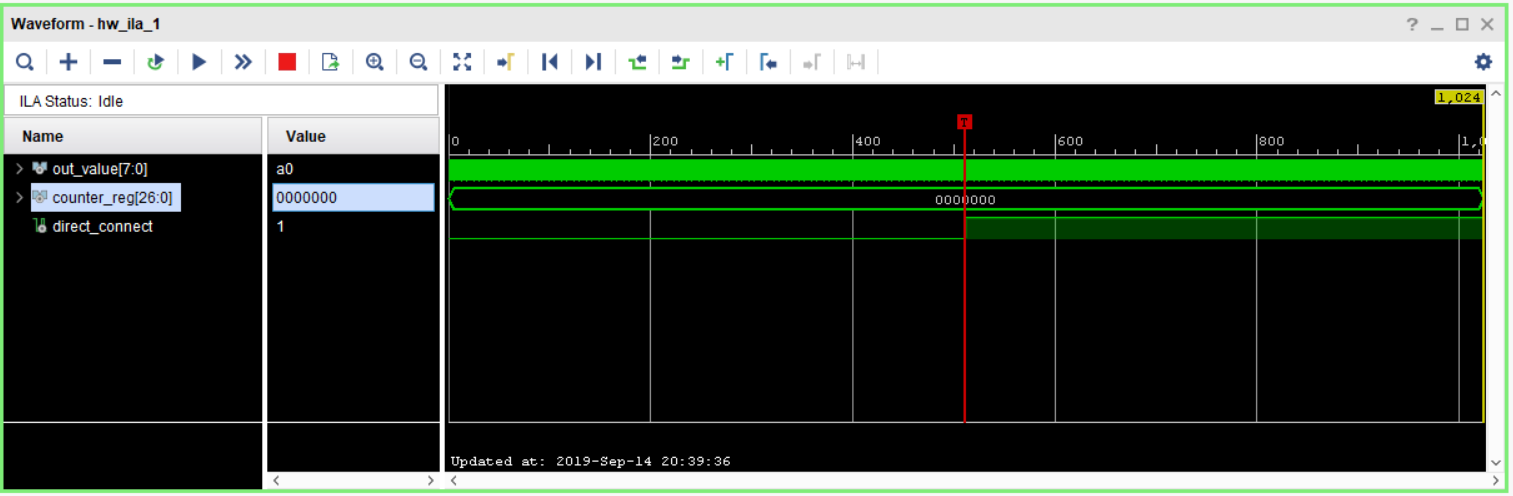
\includegraphics[width=0.9\textwidth]{images/ila_waveform.png}
    \caption{The ILA waveform output}
    \label{fig:ila_waveform}
\end{figure}




\section{ILA Core Instantiation in IP Integrator}
\label{sec:ila_core}
Previously in the tutorial, we covered the automated \textit{ILA} insertion flow using the \textit{Debug Wizard}. We can also insert an ILA core manually into our design. This later methodology tends to be the easier approach for signals within the IP Integrator environment. For this tutorial, we'll be inserting an ILA into our DDR-based MicroBlaze system of tutorial~3. \textbf{Open} the project from tutorial~3, or alternatively create a new project and recreate the system we designed there. \textbf{Open} the block diagram. Note, we can also mark a signal as debug in this view and use the flow present in Section~\ref{sec:mark_as_debug}. To see how this works, \textbf{right click} on the \textit{interrupt} output of the \textit{AXI Uartlite} and select \textbf{Debug}. If we save the block diagram now and close it, we can run the steps of Section~\ref{sec:mark_as_debug} to automatically insert the ILA. We won't be using that method in this part of the tutorial. \textbf{Right click} the signal you just marked as debug and select \textbf{Clear Debug} to remove the signal from the Debug Nets list.

Instead, we will be manually inserting an \textit{ILA}. \textbf{Right click} anywhere in the block diagram editor and select \textbf{ADD IP}. Search for and select \textit{ILA} to add a new \textit{ILA} to the project. \textbf{Double click} on the newly added \textit{ILA} to bring up its configuration window. From here, we can select between \textit{Native} and \textit{AXI} mode. The native mode has simple probes of some specified width, while the AXI mode include full AXI interfaces, which is a series of signals that implement the AXI protocol. For this section of the tutorial, we will be demonstrating the use of the AXI-based \textit{ILA}, so make sure \textbf{AXI} is selected for the \textit{Monitor Type}. Next, we can select how many probes to include. If we're using \textit{AXI} mode, we can only have a single probe (since AXI has multiple signals itself), but we can select up to 1024 individual signals in native mode. Finally, we can select the depth of the ILA; we'll leave the \textit{Sample Data Depth} at \textbf{1024} for this tutorial. See Figure~\ref{fig:ila_config} for reference. The next tab in the configuration allows us to set the parameters for each probe. The parameters for the AXI probes are deduced automatically from the design, though in native mode here is where you would select the bitwidth of each of your probes.

\begin{figure}[!h]
    \centering
    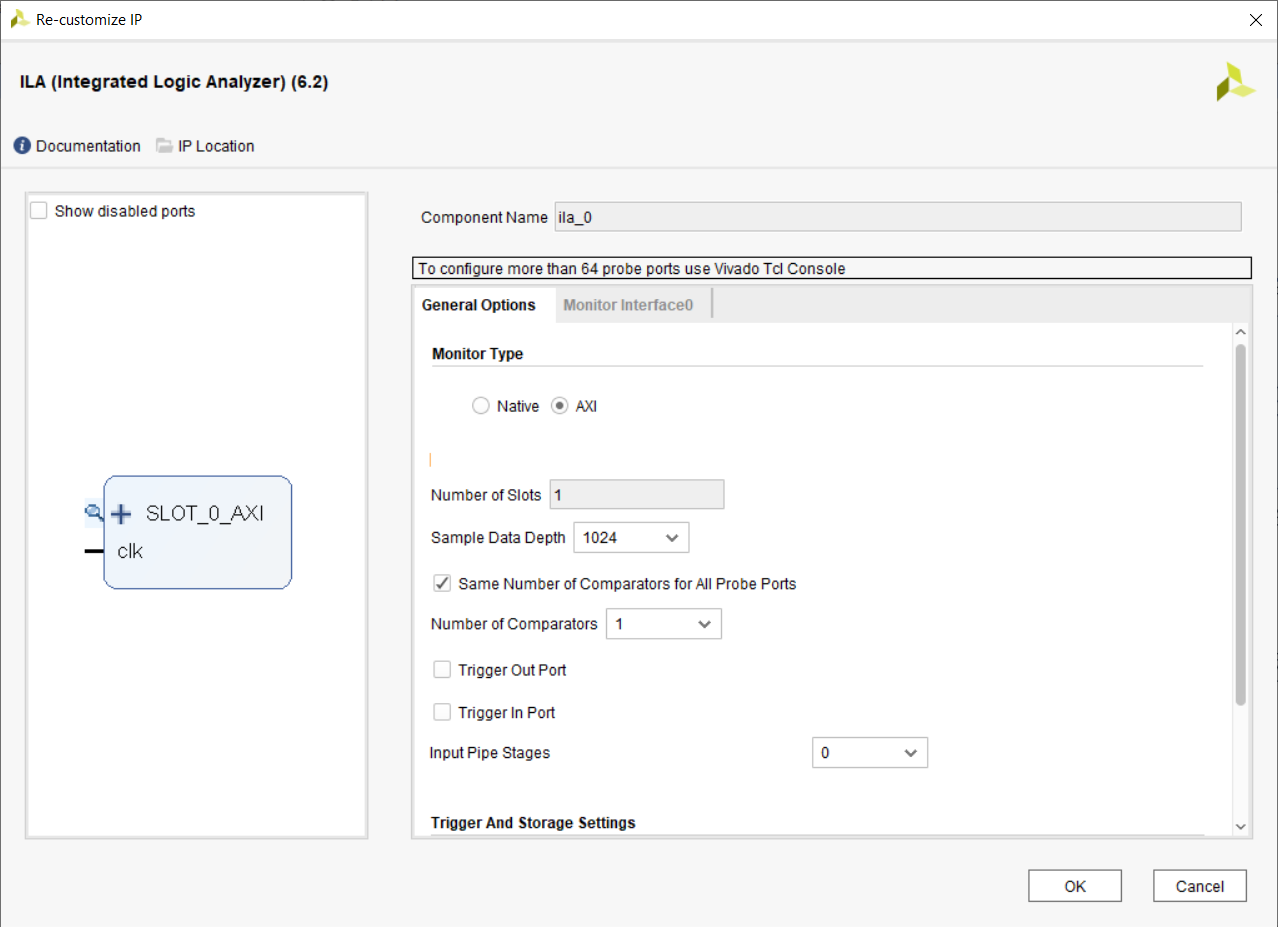
\includegraphics[width=0.95\textwidth]{images/ila_config.png}
    \caption{Configuration window for the ILA core}
    \label{fig:ila_config}
\end{figure}

Close the configuration window. \textbf{Connect} the \textit{SLOT\_0\_AXI} signal of the \textit{ILA} core to the AXI input to the \textit{MIG DDR Controller}. We also need to connect the \textit{clk} signal of the \textit{ILA} to match the clock used for this AXI interface, which is the \textit{ui\_clk} output of the \textit{MIG} itself. You should see a connectivity similar to Figure~\ref{fig:ila_connect}. Once you have an \textit{ILA} connected in the \textit{Block Diagram} editor as we've just done, there are no further steps needed to enable the debug of this signal. We can now \textbf{Save} the block diagram, run \textbf{Validate Design}, and then run \textbf{Synthesis}, \textbf{Implementation}, and \textbf{Generate Bitstream} to create the final bitstream.

\begin{figure}[!h]
    \centering
    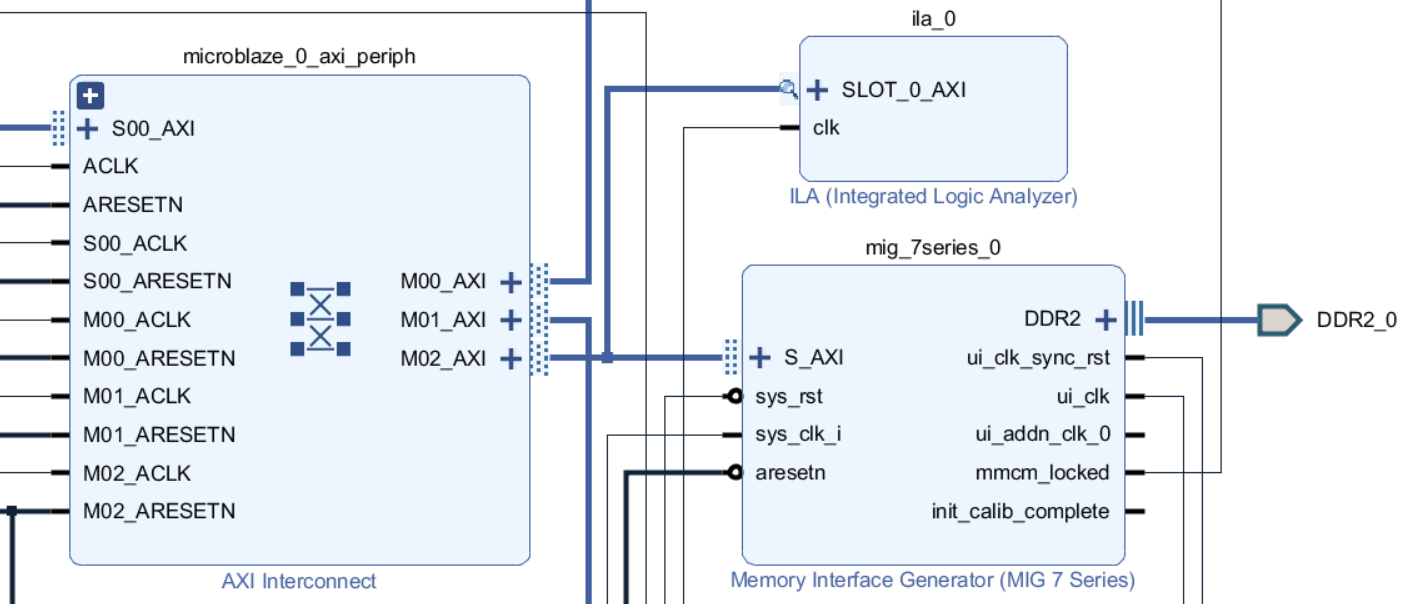
\includegraphics[width=0.9\textwidth]{images/ila_connect.png}
    \caption{The ILA core connect to the AXI interface of the MIG}
    \label{fig:ila_connect}
\end{figure}




\section{Using an ILA with an AXI Interface in Hardware Manager}
\label{sec:hw_man2}
Open \textbf{Hardware Manager} and program the FPGA with your newly created bitstream, making sure that the probes file is automatically selected for you as we did in Section~\ref{sec:hw_man}. In the \textit{Trigger Setup} tab, press
~\scalerel*{
\includegraphics{images/add_probe.png}}{(}~
button to add a new probe for a trigger event. From the list, select the AXI signal that ends in \textbf{WVALID}. Repeat this step and add the signal that ends in \textbf{WREADY}. Set the \textit{Value} field for both triggers to \textit{1 (logical one)}. These two signals correspond to the write data channel, where we expect the write data to be transmitted. The \textit{valid} signal indicates that there is valid data being transmitted, and the \textit{ready} signal indicates that the data is accepted. If we set the trigger to \textbf{global AND} by pressing the 
~\scalerel*{
\includegraphics{images/global_trigger.png}}{(}~
button, we will trigger on valid data transmitted. \textbf{Run} the \textit{ILA} to wait for  the trigger event.

We cannot trigger the event from the switches, so we have to run an application on the MicroBlaze to trigger the \textit{ILA}. Without closing the \textit{Hardware Manager}, \textbf{Export} the Hardware and start \textbf{Vivado SDK}. Open the \textit{helloworld} application created in tutorial~3. Note, sometimes when we change the MicroBlaze system, our SDK applications fail to compile. We need to refresh the include files included in the board support package; press the \textbf{Re-generate BSP Sources} button from the \textit{system.mss} window to refresh the \textit{bsp}.
%so open an include file in the \textit{hello\_bsp} directory (\textit{xil\_printf.h} for example) and press \textbf{F5} to refresh the files; you should now be able to run the application. 
Open the \textit{Run Configuration} created in tutorial~3, but don't run it quite yet. Uncheck the \textbf{Program FPGA} option and then press \textbf{Apply} (See Figure~\ref{fig:run_config_program}). We don't want to reprogram the FPGA, as that will reset our ILA. Press \textbf{Run} to run the application.

\begin{figure}[!h]
    \centering
    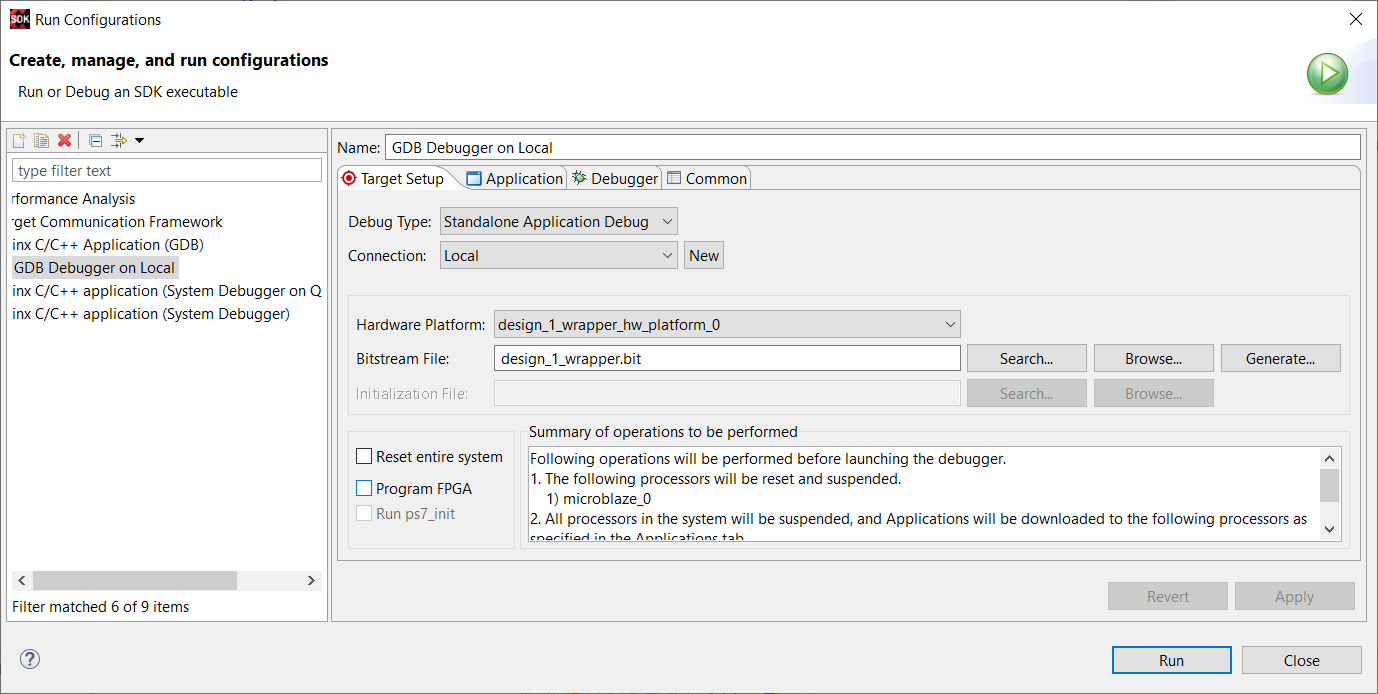
\includegraphics[width=0.95\textwidth]{images/run_config_program.png}
    \caption{Run Configuration dialog, with Program FPGA unchecked}
    \label{fig:run_config_program}
\end{figure}

Return to \textit{Hardware Manager}, the event should have triggered and we should see some output in the \textit{Waveform Viewer}. Find the signals that end in \textit{WVALID}, \textit{WREADY}, and \textit{WDATA}. You should see the values we wrote to the memory on the \textit{WDATA} signal, with subsequent values appearing after both \textit{WVALID} and \textit{WREADY} go high at the same time. 




\section{Summary}
\label{sec:summary}
The \textit{ILA} is an effective way to debug our systems as they run in real-time on the FPGAs. \textit{ILAs} can either be automatically inserted based on the Vivado Debug flow, or manual inserted as an actual \textit{ILA} core. With properly setup trigger values, we can capture our probe values when a specific event happens. The ILA can even be used in AXI mode, to capture the AXI transactions and verify the reads and writes done by AXI master devices (like the MicroBlaze).




\newpage
\printbibliography

\end{document}
